\documentclass[]{article}
\usepackage{lmodern}
\usepackage{amssymb,amsmath}
\usepackage{ifxetex,ifluatex}
\usepackage{fixltx2e} % provides \textsubscript
\ifnum 0\ifxetex 1\fi\ifluatex 1\fi=0 % if pdftex
  \usepackage[T1]{fontenc}
  \usepackage[utf8]{inputenc}
\else % if luatex or xelatex
  \ifxetex
    \usepackage{mathspec}
  \else
    \usepackage{fontspec}
  \fi
  \defaultfontfeatures{Ligatures=TeX,Scale=MatchLowercase}
\fi
% use upquote if available, for straight quotes in verbatim environments
\IfFileExists{upquote.sty}{\usepackage{upquote}}{}
% use microtype if available
\IfFileExists{microtype.sty}{%
\usepackage{microtype}
\UseMicrotypeSet[protrusion]{basicmath} % disable protrusion for tt fonts
}{}
\usepackage[margin=1in]{geometry}
\usepackage{hyperref}
\hypersetup{unicode=true,
            pdftitle={Southwest Social Networks},
            pdfauthor={Nick Gauthier},
            pdfborder={0 0 0},
            breaklinks=true}
\urlstyle{same}  % don't use monospace font for urls
\usepackage{color}
\usepackage{fancyvrb}
\newcommand{\VerbBar}{|}
\newcommand{\VERB}{\Verb[commandchars=\\\{\}]}
\DefineVerbatimEnvironment{Highlighting}{Verbatim}{commandchars=\\\{\}}
% Add ',fontsize=\small' for more characters per line
\usepackage{framed}
\definecolor{shadecolor}{RGB}{248,248,248}
\newenvironment{Shaded}{\begin{snugshade}}{\end{snugshade}}
\newcommand{\KeywordTok}[1]{\textcolor[rgb]{0.13,0.29,0.53}{\textbf{{#1}}}}
\newcommand{\DataTypeTok}[1]{\textcolor[rgb]{0.13,0.29,0.53}{{#1}}}
\newcommand{\DecValTok}[1]{\textcolor[rgb]{0.00,0.00,0.81}{{#1}}}
\newcommand{\BaseNTok}[1]{\textcolor[rgb]{0.00,0.00,0.81}{{#1}}}
\newcommand{\FloatTok}[1]{\textcolor[rgb]{0.00,0.00,0.81}{{#1}}}
\newcommand{\ConstantTok}[1]{\textcolor[rgb]{0.00,0.00,0.00}{{#1}}}
\newcommand{\CharTok}[1]{\textcolor[rgb]{0.31,0.60,0.02}{{#1}}}
\newcommand{\SpecialCharTok}[1]{\textcolor[rgb]{0.00,0.00,0.00}{{#1}}}
\newcommand{\StringTok}[1]{\textcolor[rgb]{0.31,0.60,0.02}{{#1}}}
\newcommand{\VerbatimStringTok}[1]{\textcolor[rgb]{0.31,0.60,0.02}{{#1}}}
\newcommand{\SpecialStringTok}[1]{\textcolor[rgb]{0.31,0.60,0.02}{{#1}}}
\newcommand{\ImportTok}[1]{{#1}}
\newcommand{\CommentTok}[1]{\textcolor[rgb]{0.56,0.35,0.01}{\textit{{#1}}}}
\newcommand{\DocumentationTok}[1]{\textcolor[rgb]{0.56,0.35,0.01}{\textbf{\textit{{#1}}}}}
\newcommand{\AnnotationTok}[1]{\textcolor[rgb]{0.56,0.35,0.01}{\textbf{\textit{{#1}}}}}
\newcommand{\CommentVarTok}[1]{\textcolor[rgb]{0.56,0.35,0.01}{\textbf{\textit{{#1}}}}}
\newcommand{\OtherTok}[1]{\textcolor[rgb]{0.56,0.35,0.01}{{#1}}}
\newcommand{\FunctionTok}[1]{\textcolor[rgb]{0.00,0.00,0.00}{{#1}}}
\newcommand{\VariableTok}[1]{\textcolor[rgb]{0.00,0.00,0.00}{{#1}}}
\newcommand{\ControlFlowTok}[1]{\textcolor[rgb]{0.13,0.29,0.53}{\textbf{{#1}}}}
\newcommand{\OperatorTok}[1]{\textcolor[rgb]{0.81,0.36,0.00}{\textbf{{#1}}}}
\newcommand{\BuiltInTok}[1]{{#1}}
\newcommand{\ExtensionTok}[1]{{#1}}
\newcommand{\PreprocessorTok}[1]{\textcolor[rgb]{0.56,0.35,0.01}{\textit{{#1}}}}
\newcommand{\AttributeTok}[1]{\textcolor[rgb]{0.77,0.63,0.00}{{#1}}}
\newcommand{\RegionMarkerTok}[1]{{#1}}
\newcommand{\InformationTok}[1]{\textcolor[rgb]{0.56,0.35,0.01}{\textbf{\textit{{#1}}}}}
\newcommand{\WarningTok}[1]{\textcolor[rgb]{0.56,0.35,0.01}{\textbf{\textit{{#1}}}}}
\newcommand{\AlertTok}[1]{\textcolor[rgb]{0.94,0.16,0.16}{{#1}}}
\newcommand{\ErrorTok}[1]{\textcolor[rgb]{0.64,0.00,0.00}{\textbf{{#1}}}}
\newcommand{\NormalTok}[1]{{#1}}
\usepackage{graphicx,grffile}
\makeatletter
\def\maxwidth{\ifdim\Gin@nat@width>\linewidth\linewidth\else\Gin@nat@width\fi}
\def\maxheight{\ifdim\Gin@nat@height>\textheight\textheight\else\Gin@nat@height\fi}
\makeatother
% Scale images if necessary, so that they will not overflow the page
% margins by default, and it is still possible to overwrite the defaults
% using explicit options in \includegraphics[width, height, ...]{}
\setkeys{Gin}{width=\maxwidth,height=\maxheight,keepaspectratio}
\IfFileExists{parskip.sty}{%
\usepackage{parskip}
}{% else
\setlength{\parindent}{0pt}
\setlength{\parskip}{6pt plus 2pt minus 1pt}
}
\setlength{\emergencystretch}{3em}  % prevent overfull lines
\providecommand{\tightlist}{%
  \setlength{\itemsep}{0pt}\setlength{\parskip}{0pt}}
\setcounter{secnumdepth}{0}
% Redefines (sub)paragraphs to behave more like sections
\ifx\paragraph\undefined\else
\let\oldparagraph\paragraph
\renewcommand{\paragraph}[1]{\oldparagraph{#1}\mbox{}}
\fi
\ifx\subparagraph\undefined\else
\let\oldsubparagraph\subparagraph
\renewcommand{\subparagraph}[1]{\oldsubparagraph{#1}\mbox{}}
\fi

%%% Use protect on footnotes to avoid problems with footnotes in titles
\let\rmarkdownfootnote\footnote%
\def\footnote{\protect\rmarkdownfootnote}

%%% Change title format to be more compact
\usepackage{titling}

% Create subtitle command for use in maketitle
\newcommand{\subtitle}[1]{
  \posttitle{
    \begin{center}\large#1\end{center}
    }
}

\setlength{\droptitle}{-2em}
  \title{Southwest Social Networks}
  \pretitle{\vspace{\droptitle}\centering\huge}
  \posttitle{\par}
  \author{Nick Gauthier}
  \preauthor{\centering\large\emph}
  \postauthor{\par}
  \date{}
  \predate{}\postdate{}


\begin{document}
\maketitle

\section{Data import}\label{data-import}

First import the SWSN attribute file. Use tidyverse packages for data
munging.

Site coordinates are in UTM, so first use rgdal to reproject to LatLon.

\begin{Shaded}
\begin{Highlighting}[]
\KeywordTok{library}\NormalTok{(tidyverse)}
\KeywordTok{library}\NormalTok{(rgdal)}

\NormalTok{swsn.pts <-}\StringTok{ }\KeywordTok{read_csv}\NormalTok{(}\StringTok{'Data/attributes_orig.csv'}\NormalTok{) %>%}\StringTok{ }
\StringTok{  }\KeywordTok{select}\NormalTok{(}\DataTypeTok{easting =} \NormalTok{EASTING, }\DataTypeTok{northing =} \NormalTok{NORTHING) %>%}
\StringTok{  }\KeywordTok{SpatialPoints}\NormalTok{(}\DataTypeTok{proj4string=}\KeywordTok{CRS}\NormalTok{(}\StringTok{"+proj=utm +zone=12 +datum=WGS84"}\NormalTok{)) %>%}
\StringTok{  }\KeywordTok{spTransform}\NormalTok{(}\KeywordTok{CRS}\NormalTok{(}\StringTok{"+proj=longlat +datum=WGS84"}\NormalTok{)) %>%}\StringTok{ }
\StringTok{  }\NormalTok{coordinates %>%}
\StringTok{  }\NormalTok{data.frame}
\end{Highlighting}
\end{Shaded}

Now reimport the attribute file, select the relevant data, and combine
with the reprojected site coordinates.

\begin{Shaded}
\begin{Highlighting}[]
\NormalTok{swsn.attr <-}\StringTok{ }\KeywordTok{read_csv}\NormalTok{(}\StringTok{'Data/attributes_orig.csv'}\NormalTok{) %>%}
\StringTok{  }\KeywordTok{select}\NormalTok{(}\DataTypeTok{ID =} \NormalTok{SWSN_ID, }\DataTypeTok{site =} \NormalTok{SWSN_Site, }\DataTypeTok{macro =} \NormalTok{Macro, }\DataTypeTok{micro =} \NormalTok{Micro) %>%}
\StringTok{  }\KeywordTok{cbind}\NormalTok{(swsn.pts)}
\end{Highlighting}
\end{Shaded}

Now define a function to import the SWSN adjacency matrix for a given
time step. This function imports the adjacency matrix, keeps only those
connections with \textgreater{}= 75\% similarity, and creates an igraph
object. Then it adds attribute data from above to the graph object.

\begin{Shaded}
\begin{Highlighting}[]
\KeywordTok{library}\NormalTok{(igraph)}

\NormalTok{readSWSN <-}\StringTok{ }\NormalTok{function(net)\{}
  \NormalTok{net.in <-}\StringTok{ }\KeywordTok{read.csv}\NormalTok{(net, }\DataTypeTok{row.names =} \DecValTok{1}\NormalTok{, }\DataTypeTok{check.names =} \NormalTok{F) }
  \NormalTok{net.in[net.in <}\StringTok{ }\NormalTok{.}\DecValTok{75}\NormalTok{] <-}\StringTok{ }\DecValTok{0}
  \NormalTok{net.in <-}\StringTok{ }\NormalTok{net.in %>%}\StringTok{ }
\StringTok{    }\NormalTok{as.matrix %>%}
\StringTok{    }\KeywordTok{graph_from_adjacency_matrix}\NormalTok{(}\DataTypeTok{mode =} \StringTok{'undirected'}\NormalTok{, }\DataTypeTok{weighted =} \NormalTok{T, }\DataTypeTok{diag =} \NormalTok{F)}
  
  \NormalTok{ord <-}\StringTok{ }\KeywordTok{match}\NormalTok{(}\KeywordTok{V}\NormalTok{(net.in)$name, swsn.attr$site)}

  \KeywordTok{V}\NormalTok{(net.in)$lon <-}\StringTok{ }\NormalTok{swsn.attr[ord, }\DecValTok{5}\NormalTok{]}
  \KeywordTok{V}\NormalTok{(net.in)$lat <-}\StringTok{ }\NormalTok{swsn.attr[ord, }\DecValTok{6}\NormalTok{]}
  \KeywordTok{V}\NormalTok{(net.in)$region <-}\StringTok{ }\NormalTok{swsn.attr[ord, }\DecValTok{3}\NormalTok{] %>%}\StringTok{ }\NormalTok{as.character}
  
  \KeywordTok{return}\NormalTok{(net.in)}
\NormalTok{\}}
\end{Highlighting}
\end{Shaded}

Use the function to import the network datasets.

\begin{Shaded}
\begin{Highlighting}[]
\NormalTok{ad1200 <-}\StringTok{ }\KeywordTok{readSWSN}\NormalTok{(}\StringTok{'Data/AD1200sim.csv'}\NormalTok{)}
\NormalTok{ad1250 <-}\StringTok{ }\KeywordTok{readSWSN}\NormalTok{(}\StringTok{'Data/AD1250sim.csv'}\NormalTok{)}
\NormalTok{ad1300 <-}\StringTok{ }\KeywordTok{readSWSN}\NormalTok{(}\StringTok{'Data/AD1300sim.csv'}\NormalTok{)}
\NormalTok{ad1350 <-}\StringTok{ }\KeywordTok{readSWSN}\NormalTok{(}\StringTok{'Data/AD1350sim.csv'}\NormalTok{)}
\NormalTok{ad1400 <-}\StringTok{ }\KeywordTok{readSWSN}\NormalTok{(}\StringTok{'Data/AD1400sim.csv'}\NormalTok{)}
\end{Highlighting}
\end{Shaded}

\section{Plotting}\label{plotting}

First get a terrain basemap to plot the networks over. The
terrain-background basemap from Stamen is a nice choice. Download this
map and store a ggmap plot of it.

\begin{Shaded}
\begin{Highlighting}[]
\KeywordTok{library}\NormalTok{(ggmap)}
\NormalTok{terrain.background <-}\StringTok{ }\KeywordTok{get_map}\NormalTok{(}\DataTypeTok{location =} \KeywordTok{c}\NormalTok{(}\DataTypeTok{left =} \NormalTok{-}\FloatTok{113.5}\NormalTok{, }\DataTypeTok{right =} \NormalTok{-}\FloatTok{106.5}\NormalTok{, }\DataTypeTok{bottom =} \DecValTok{31}\NormalTok{, }\DataTypeTok{top =} \FloatTok{37.5}\NormalTok{),}
  \DataTypeTok{zoom =} \DecValTok{8}\NormalTok{,}
  \DataTypeTok{color =} \StringTok{"color"}\NormalTok{,}
  \DataTypeTok{source =} \StringTok{"stamen"}\NormalTok{,}
  \DataTypeTok{maptype =} \StringTok{"terrain-background"}\NormalTok{)}

\NormalTok{map <-}\StringTok{ }\KeywordTok{ggmap}\NormalTok{(terrain.background)  +}
\StringTok{  }\KeywordTok{labs}\NormalTok{(}\DataTypeTok{x =} \StringTok{"Longitude"}\NormalTok{, }\DataTypeTok{y =} \StringTok{"Latitude"}\NormalTok{)}
\end{Highlighting}
\end{Shaded}

Now plot the networks.

\subsection{More Minimal network maps}\label{more-minimal-network-maps}

\begin{Shaded}
\begin{Highlighting}[]
\KeywordTok{library}\NormalTok{(GGally)}
\end{Highlighting}
\end{Shaded}

\begin{verbatim}
## 
## Attaching package: 'GGally'
\end{verbatim}

\begin{verbatim}
## The following object is masked from 'package:dplyr':
## 
##     nasa
\end{verbatim}

\begin{Shaded}
\begin{Highlighting}[]
\KeywordTok{library}\NormalTok{(ggmap)}
\end{Highlighting}
\end{Shaded}

\begin{verbatim}
## Google Maps API Terms of Service: http://developers.google.com/maps/terms.
\end{verbatim}

\begin{verbatim}
## Please cite ggmap if you use it: see citation("ggmap") for details.
\end{verbatim}

\begin{Shaded}
\begin{Highlighting}[]
\KeywordTok{library}\NormalTok{(maps)}
\end{Highlighting}
\end{Shaded}

\begin{verbatim}
## 
## Attaching package: 'maps'
\end{verbatim}

\begin{verbatim}
## The following object is masked from 'package:purrr':
## 
##     map
\end{verbatim}

\begin{Shaded}
\begin{Highlighting}[]
\KeywordTok{library}\NormalTok{(raster)}
\end{Highlighting}
\end{Shaded}

\begin{verbatim}
## 
## Attaching package: 'raster'
\end{verbatim}

\begin{verbatim}
## The following object is masked from 'package:dplyr':
## 
##     select
\end{verbatim}

\begin{verbatim}
## The following object is masked from 'package:tidyr':
## 
##     extract
\end{verbatim}

\begin{Shaded}
\begin{Highlighting}[]
\KeywordTok{library}\NormalTok{(maptools)}
\end{Highlighting}
\end{Shaded}

\begin{verbatim}
## Checking rgeos availability: TRUE
\end{verbatim}

\begin{Shaded}
\begin{Highlighting}[]
\NormalTok{states <-}\StringTok{ }\KeywordTok{map}\NormalTok{(}\StringTok{'state'}\NormalTok{, }\DataTypeTok{regions =} \KeywordTok{c}\NormalTok{(}\StringTok{'arizona'}\NormalTok{, }\StringTok{'new mexico'}\NormalTok{), }\DataTypeTok{fill =} \NormalTok{T, }\DataTypeTok{plot =} \NormalTok{F)}
\NormalTok{IDs <-}\StringTok{ }\KeywordTok{sapply}\NormalTok{(}\KeywordTok{strsplit}\NormalTok{(states$names, }\StringTok{":"}\NormalTok{), function(x) x[}\DecValTok{1}\NormalTok{])}
\NormalTok{states.ply <-}\StringTok{ }\KeywordTok{map2SpatialPolygons}\NormalTok{(states, }\DataTypeTok{IDs=}\NormalTok{IDs)}



\NormalTok{base <-}\StringTok{ }\KeywordTok{ggplot}\NormalTok{(}\DataTypeTok{data =} \NormalTok{states) +}
\StringTok{  }\KeywordTok{geom_polygon}\NormalTok{(}\KeywordTok{aes}\NormalTok{(}\DataTypeTok{x =} \NormalTok{long, }\DataTypeTok{y =} \NormalTok{lat, }\DataTypeTok{group =} \NormalTok{region), }\DataTypeTok{color =} \StringTok{'black'}\NormalTok{, }\DataTypeTok{fill =} \StringTok{'white'}\NormalTok{) +}
\StringTok{  }\KeywordTok{coord_quickmap}\NormalTok{() +}
\StringTok{  }\KeywordTok{theme_minimal}\NormalTok{() +}
\StringTok{  }\KeywordTok{labs}\NormalTok{(}\DataTypeTok{x =} \StringTok{"Longitude"}\NormalTok{, }\DataTypeTok{y =} \StringTok{"Latitude"}\NormalTok{)}

\NormalTok{n1 <-}\StringTok{ }\KeywordTok{ggnetworkmap}\NormalTok{(base, ad1200, }\DataTypeTok{great.circles =} \NormalTok{T, }\DataTypeTok{size =} \NormalTok{.}\DecValTok{5}\NormalTok{, }\DataTypeTok{segment.alpha =} \KeywordTok{I}\NormalTok{(.}\DecValTok{5}\NormalTok{)) +}
\StringTok{  }\KeywordTok{geom_label}\NormalTok{(}\DataTypeTok{x =} \NormalTok{-}\DecValTok{106}\NormalTok{, }\DataTypeTok{y =} \DecValTok{35}\NormalTok{, }\DataTypeTok{label =} \StringTok{'AD 1200'}\NormalTok{)}
\end{Highlighting}
\end{Shaded}

\begin{verbatim}
## Loading required package: network
\end{verbatim}

\begin{verbatim}
## network: Classes for Relational Data
## Version 1.13.0 created on 2015-08-31.
## copyright (c) 2005, Carter T. Butts, University of California-Irvine
##                     Mark S. Handcock, University of California -- Los Angeles
##                     David R. Hunter, Penn State University
##                     Martina Morris, University of Washington
##                     Skye Bender-deMoll, University of Washington
##  For citation information, type citation("network").
##  Type help("network-package") to get started.
\end{verbatim}

\begin{verbatim}
## 
## Attaching package: 'network'
\end{verbatim}

\begin{verbatim}
## The following objects are masked from 'package:igraph':
## 
##     add.edges, add.vertices, %c%, delete.edges, delete.vertices,
##     get.edge.attribute, get.edges, get.vertex.attribute,
##     is.bipartite, is.directed, list.edge.attributes,
##     list.vertex.attributes, %s%, set.edge.attribute,
##     set.vertex.attribute
\end{verbatim}

\begin{verbatim}
## Loading required package: sna
\end{verbatim}

\begin{verbatim}
## Loading required package: statnet.common
\end{verbatim}

\begin{verbatim}
## sna: Tools for Social Network Analysis
## Version 2.4 created on 2016-07-23.
## copyright (c) 2005, Carter T. Butts, University of California-Irvine
##  For citation information, type citation("sna").
##  Type help(package="sna") to get started.
\end{verbatim}

\begin{verbatim}
## 
## Attaching package: 'sna'
\end{verbatim}

\begin{verbatim}
## The following objects are masked from 'package:igraph':
## 
##     betweenness, bonpow, closeness, components, degree,
##     dyad.census, evcent, hierarchy, is.connected, neighborhood,
##     triad.census
\end{verbatim}

\begin{verbatim}
## Loading required package: geosphere
\end{verbatim}

\begin{Shaded}
\begin{Highlighting}[]
\NormalTok{n2 <-}\StringTok{ }\KeywordTok{ggnetworkmap}\NormalTok{(base, ad1250, }\DataTypeTok{great.circles =} \NormalTok{T, }\DataTypeTok{size =} \NormalTok{.}\DecValTok{5}\NormalTok{, }\DataTypeTok{segment.alpha =} \KeywordTok{I}\NormalTok{(.}\DecValTok{5}\NormalTok{)) +}
\StringTok{  }\KeywordTok{geom_label}\NormalTok{(}\DataTypeTok{x =} \NormalTok{-}\DecValTok{106}\NormalTok{, }\DataTypeTok{y =} \DecValTok{35}\NormalTok{, }\DataTypeTok{label =} \StringTok{'AD 1250'}\NormalTok{)}

\NormalTok{n3 <-}\StringTok{ }\KeywordTok{ggnetworkmap}\NormalTok{(base, ad1300, }\DataTypeTok{great.circles =} \NormalTok{T, }\DataTypeTok{size =} \NormalTok{.}\DecValTok{5}\NormalTok{, }\DataTypeTok{segment.alpha =} \KeywordTok{I}\NormalTok{(.}\DecValTok{5}\NormalTok{)) +}
\StringTok{  }\KeywordTok{geom_label}\NormalTok{(}\DataTypeTok{x =} \NormalTok{-}\DecValTok{106}\NormalTok{, }\DataTypeTok{y =} \DecValTok{35}\NormalTok{, }\DataTypeTok{label =} \StringTok{'AD 1300'}\NormalTok{)}

\NormalTok{n4 <-}\StringTok{ }\KeywordTok{ggnetworkmap}\NormalTok{(base, ad1350, }\DataTypeTok{great.circles =} \NormalTok{T, }\DataTypeTok{size =} \NormalTok{.}\DecValTok{5}\NormalTok{, }\DataTypeTok{segment.alpha =} \KeywordTok{I}\NormalTok{(.}\DecValTok{5}\NormalTok{)) +}
\StringTok{  }\KeywordTok{geom_label}\NormalTok{(}\DataTypeTok{x =} \NormalTok{-}\DecValTok{106}\NormalTok{, }\DataTypeTok{y =} \DecValTok{35}\NormalTok{, }\DataTypeTok{label =} \StringTok{'AD 1350'}\NormalTok{)}

\NormalTok{n5 <-}\StringTok{ }\KeywordTok{ggnetworkmap}\NormalTok{(base, ad1400, }\DataTypeTok{great.circles =} \NormalTok{T, }\DataTypeTok{size =} \NormalTok{.}\DecValTok{5}\NormalTok{, }\DataTypeTok{segment.alpha =} \KeywordTok{I}\NormalTok{(.}\DecValTok{5}\NormalTok{)) +}
\StringTok{  }\KeywordTok{geom_label}\NormalTok{(}\DataTypeTok{x =} \NormalTok{-}\DecValTok{106}\NormalTok{, }\DataTypeTok{y =} \DecValTok{35}\NormalTok{, }\DataTypeTok{label =} \StringTok{'AD 1400'}\NormalTok{)}

\NormalTok{plotEOF <-}\StringTok{ }\NormalTok{function(x)\{}
  \NormalTok{rasterVis::}\KeywordTok{gplot}\NormalTok{(x) +}
\StringTok{  }\KeywordTok{geom_raster}\NormalTok{(}\KeywordTok{aes}\NormalTok{(}\DataTypeTok{fill =} \NormalTok{value), }\DataTypeTok{na.rm =} \NormalTok{T, }\DataTypeTok{show.legend =} \NormalTok{F) +}
\StringTok{  }\KeywordTok{scale_fill_distiller}\NormalTok{(}\DataTypeTok{palette =} \StringTok{'RdBu'}\NormalTok{, }\DataTypeTok{na.value =} \OtherTok{NA}\NormalTok{) +}
\StringTok{  }\KeywordTok{geom_polygon}\NormalTok{(}\DataTypeTok{data =} \NormalTok{states, }\KeywordTok{aes}\NormalTok{(}\DataTypeTok{x =} \NormalTok{long, }\DataTypeTok{y =} \NormalTok{lat, }\DataTypeTok{group =} \NormalTok{region), }\DataTypeTok{color =} \StringTok{'black'}\NormalTok{, }\DataTypeTok{fill =} \OtherTok{NA}\NormalTok{) +}
\StringTok{  }\KeywordTok{coord_quickmap}\NormalTok{() +}
\StringTok{  }\KeywordTok{theme_minimal}\NormalTok{() +}
\StringTok{  }\KeywordTok{labs}\NormalTok{(}\DataTypeTok{x =} \StringTok{"Longitude"}\NormalTok{, }\DataTypeTok{y =} \StringTok{"Latitude"}\NormalTok{)}
\NormalTok{\}}

\NormalTok{eof1200 <-}\StringTok{ }\KeywordTok{brick}\NormalTok{(}\StringTok{'Data/eof1200.nc'}\NormalTok{)[[}\DecValTok{3}\NormalTok{]] %>%}
\StringTok{  }\KeywordTok{mask}\NormalTok{(states.ply) %>%}\StringTok{ }
\StringTok{  }\NormalTok{plotEOF}
\end{Highlighting}
\end{Shaded}

\begin{verbatim}
## Loading required namespace: ncdf4
\end{verbatim}

\begin{Shaded}
\begin{Highlighting}[]
\NormalTok{e1 <-}\StringTok{ }\KeywordTok{ggnetworkmap}\NormalTok{(eof1200, ad1200, }\DataTypeTok{great.circles =} \NormalTok{T, }\DataTypeTok{size =} \NormalTok{.}\DecValTok{5}\NormalTok{, }\DataTypeTok{segment.alpha =} \KeywordTok{I}\NormalTok{(.}\DecValTok{5}\NormalTok{)) }\CommentTok{#+ geom_label(x = -106, y = 35, label = 'AD 1200')}

  
\NormalTok{eof1250 <-}\StringTok{ }\KeywordTok{brick}\NormalTok{(}\StringTok{'Data/eof1250.nc'}\NormalTok{)[[}\DecValTok{3}\NormalTok{]] %>%}
\StringTok{  }\KeywordTok{mask}\NormalTok{(states.ply) %>%}
\StringTok{    }\NormalTok{plotEOF}


\NormalTok{e2 <-}\StringTok{ }\KeywordTok{ggnetworkmap}\NormalTok{(eof1250, ad1250, }\DataTypeTok{great.circles =} \NormalTok{T, }\DataTypeTok{size =} \NormalTok{.}\DecValTok{5}\NormalTok{, }\DataTypeTok{segment.alpha =} \KeywordTok{I}\NormalTok{(.}\DecValTok{5}\NormalTok{)) }\CommentTok{#+  geom_label(x = -106, y = 35, label = 'AD 1250')}

\NormalTok{eof1300 <-}\StringTok{ }\KeywordTok{brick}\NormalTok{(}\StringTok{'Data/eof1300.nc'}\NormalTok{)[[}\DecValTok{3}\NormalTok{]] %>%}
\StringTok{  }\KeywordTok{mask}\NormalTok{(states.ply) %>%}
\StringTok{    }\NormalTok{plotEOF}

\NormalTok{e3 <-}\StringTok{ }\KeywordTok{ggnetworkmap}\NormalTok{(eof1300, ad1300, }\DataTypeTok{great.circles =} \NormalTok{T, }\DataTypeTok{size =} \NormalTok{.}\DecValTok{5}\NormalTok{, }\DataTypeTok{segment.alpha =} \KeywordTok{I}\NormalTok{(.}\DecValTok{5}\NormalTok{))}\CommentTok{# + geom_label(x = -106, y = 35, label = 'AD 1300')}

\NormalTok{eof1350 <-}\StringTok{ }\KeywordTok{brick}\NormalTok{(}\StringTok{'Data/eof1350.nc'}\NormalTok{)[[}\DecValTok{3}\NormalTok{]] %>%}
\StringTok{  }\KeywordTok{mask}\NormalTok{(states.ply) %>%}
\StringTok{    }\NormalTok{plotEOF}

\NormalTok{e4 <-}\StringTok{ }\KeywordTok{ggnetworkmap}\NormalTok{(eof1350, ad1350, }\DataTypeTok{great.circles =} \NormalTok{T, }\DataTypeTok{size =} \NormalTok{.}\DecValTok{5}\NormalTok{, }\DataTypeTok{segment.alpha =} \KeywordTok{I}\NormalTok{(.}\DecValTok{5}\NormalTok{)) }\CommentTok{#+ geom_label(x = -106, y = 35, label = 'AD 1350')}

\NormalTok{eof1400 <-}\StringTok{ }\KeywordTok{brick}\NormalTok{(}\StringTok{'Data/eof1400.nc'}\NormalTok{)[[}\DecValTok{3}\NormalTok{]] %>%}
\StringTok{  }\KeywordTok{mask}\NormalTok{(states.ply) %>%}
\StringTok{    }\NormalTok{plotEOF}

\NormalTok{e5 <-}\StringTok{ }\KeywordTok{ggnetworkmap}\NormalTok{(eof1400, ad1400, }\DataTypeTok{great.circles =} \NormalTok{T, }\DataTypeTok{size =} \NormalTok{.}\DecValTok{5}\NormalTok{, }\DataTypeTok{segment.alpha =} \KeywordTok{I}\NormalTok{(.}\DecValTok{5}\NormalTok{)) }\CommentTok{#+ geom_label(x = -106, y = 35, label = 'AD 1400')}
\end{Highlighting}
\end{Shaded}

Get basemap for elevation.

\begin{Shaded}
\begin{Highlighting}[]
\CommentTok{#multiplot(n1, n2, n3, n4, layout = matrix(c(1,2,3,4), byrow = T, nrow = 2))}
\KeywordTok{multiplot}\NormalTok{(e1, e2, e3, e4, }\DataTypeTok{layout =} \KeywordTok{matrix}\NormalTok{(}\KeywordTok{c}\NormalTok{(}\DecValTok{1}\NormalTok{,}\DecValTok{2}\NormalTok{,}\DecValTok{3}\NormalTok{,}\DecValTok{4}\NormalTok{), }\DataTypeTok{byrow =} \NormalTok{T, }\DataTypeTok{nrow =} \DecValTok{2}\NormalTok{))}
\end{Highlighting}
\end{Shaded}

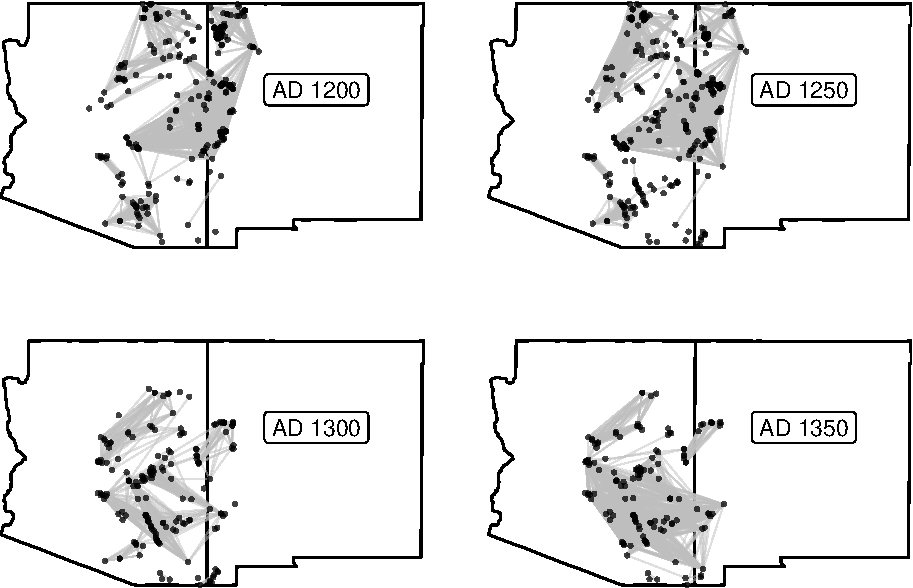
\includegraphics{network_files/figure-latex/unnamed-chunk-10-1.pdf}

\begin{Shaded}
\begin{Highlighting}[]
\CommentTok{#multiplot(n1, n2, n3, n4, n5, m1, layout = matrix(c(1,2,3,4,5,6), byrow = T, nrow = 3))}
\CommentTok{#multiplot(e1, e2, e3, e4, e5, layout = matrix(c(1,2,3,4,5,6), byrow = T, nrow = 3))}
\end{Highlighting}
\end{Shaded}

eof1200 \textless{}- brick(`Data/eof1200.nc'){[}{[}4{]}{]}
\%\textgreater{}\% mask(states.ply) \%\textgreater{}\% plotEOF

e1 \textless{}- ggnetworkmap(eof1200, ad1200, great.circles = T, size =
.5, segment.alpha = I(.5)) + geom\_label(x = -106, y = 35, label = `AD
1200')

eof1250 \textless{}- brick(`Data/eof1250.nc'){[}{[}4{]}{]}
\%\textgreater{}\% mask(states.ply) \%\textgreater{}\% plotEOF

e2 \textless{}- ggnetworkmap(eof1250, ad1250, great.circles = T, size =
.5, segment.alpha = I(.5)) + geom\_label(x = -106, y = 35, label = `AD
1250')

eof1300 \textless{}- brick(`Data/eof1300.nc'){[}{[}4{]}{]}
\%\textgreater{}\% mask(states.ply) \%\textgreater{}\% plotEOF

e3 \textless{}- ggnetworkmap(eof1300, ad1300, great.circles = T, size =
.5, segment.alpha = I(.5)) + geom\_label(x = -106, y = 35, label = `AD
1300')

eof1350 \textless{}- brick(`Data/eof1350.nc'){[}{[}4{]}{]}
\%\textgreater{}\% mask(states.ply) \%\textgreater{}\% plotEOF

multiplot(e1, e2, e3, e4, layout = matrix(c(1,2,3,4), byrow = T, nrow =
2))


\end{document}
